\documentclass[a4paper,12pt]{article}
\usepackage{geometry}
\usepackage{enumitem}
\usepackage{fancyhdr}
\usepackage{xcolor}
\usepackage{sectsty}
\usepackage{multicol}
\usepackage{graphicx}
\usepackage{amsmath}
\usepackage{float}
\def\inputGnumericTable{}
\usepackage[latin1]{inputenc}
\usepackage{fullpage}
\usepackage{color}
\usepackage{array}
\usepackage{longtable}
\usepackage{calc}
\usepackage{multirow}
\usepackage{hhline}
\usepackage{ifthen}
\geometry{top=1in, bottom=1.5cm, left=1.5cm, right=1.5cm}    % Header and Footer settings
\pagestyle{empty}
\sectionfont{\color{blue}}
\begin{document}

\thispagestyle{fancy}
\fancyhf{} % Clear default header and footer
\fancyhead[L]{% Left header
        
\includegraphics[width=8cm, height=1.7cm]{IIITB-COMET-Logo.png} % Adjust dimensions
}
\fancyhead[R]{% Right header
    Name: N.Srinivas \\
    Batch: COMETFWC036 \\
    Date: 29 August 2025
}
\renewcommand{\headrulewidth}{0pt} % Remove header line
\fancyfoot[C]{\thepage} % Page number centered in footer
\vspace*{1cm}
\begin{center}
	{\LARGE \textbf{\textcolor{blue}{GATE 2010 CS, $6^{th}$ Question Analysis}}}
\end{center}
\section*{\textbf{Question 6}}
The minterm expression of $F(P,Q,R)=PQ+Q\bar{R}+P\bar{R}$
\section*{\textbf{Question Analysis:}}
\textbf{Finding minterms of the expression $F=PQ+Q\bar{R}+P\bar{R}$}

\textbf{Step 1: Write the expression}
$
F = PQ +Q\bar{R} + P\bar{R}
$

\textbf{Step 2: Expand each term to include all variables \(P, Q, R\)}
$$
\begin{aligned}
PQ = PQ(R +\bar{R}) = PQR + PQ\bar{R} \\
Q\bar{R}= (P +\bar{P})Q\bar{R} = PQ\bar{R} + \bar{P}Q\bar{R} \\
P\bar{R}= (Q + \bar{Q})P\bar{R} = PQ\bar{R} + P\bar{Q}\bar{R}
\end{aligned}
$$

\textbf{Step 3: Combine all terms (removing duplicates)}
$
F =PQR + PQ\bar{R} + \bar{P}Q\bar{R} + P\bar{Q}\bar{R}
$

Note that \(\bar{P} Q \bar{R}\) is the same as \(\bar{P} Q \bar{R}\).

\textbf{Step 4: Identify minterms explicitly from each product}

$$
\begin{array}{c|c|c|c}
\text{Term} & \text{Minterms (binary)} & \text{Decimal} \\
\hline
PQ & P Q R = 111, \quad P Q \bar{R} = 110 & 7, 6 \\
Q\bar{R} & P Q \bar{R} = 110, \quad \bar{P} Q \bar{R} = 010 & 6, 2 \\
P\bar{R} & P Q \bar{R} = 110, \quad P \bar{Q} \bar{R} = 100 & 6, 4 \\
\end{array}
$$

\textbf{Step 5: Unique minterms}

$
m_2, \quad m_4, \quad m_6, \quad m_7
$

\textbf{Step 6: Final expression in sum of minterms notation}

$
f = \sum m(2, 4, 6, 7)
$

\section*{\textbf{Hardware Implementation}}
The above problem is implemented and tested in hardware using Arduino UNO board. Here we implemented a FSM using the 7474 IC and blinked the LED as per truth table and verified the expression.
\section*{Required Components \& Pin Connections}
\begin{center}
\begin{minipage}{0.45\textwidth}
\begin{table}[H]
\centering
\begin{tabular}{|c|l|}
\hline
\textbf{S.No} & \textbf{Component} \\ \hline
1 & Arduino Uno Board \\
2 & Breadboard \\
4 & LEDs (1) \\
7 & Resistors: 220$\Omega$ (2) \\
8 & Jumper Wires \\
9 & USB Cable \\
\hline
\end{tabular}
\end{table}
\end{minipage}
\hspace{0.05\textwidth}
\begin{minipage}{0.45\textwidth}
\begin{table}[H]
\centering
\begin{tabular}{|c|c|}
\hline
\textbf{Component} & \textbf{Arduino Pin} \\ \hline
Input P  & Digital 2 \\
Input Q  & Digital 3 \\
Input R  & Digital 4 \\
Output F (LED) & Digital 7 \\
GND & GND \\
VCC & 5V \\
\hline
\end{tabular}
\end{table}
\end{minipage}
\end{center}
\section*{Logic Description}
\begin{itemize}
	\item Let initialize inputs $A=0,B=0,C=0$
	\item The output expressions from truth table is:
	\begin{multicols}{2}	
	\item $F=P\bar{R}+Q\bar{R}+PQ$
	\end{multicols}
\end{itemize}
\section*{Code Uploading Steps}
\begin{enumerate}
	\item Create a Platform IO project
	\item Write The code in main.cpp in src
	\item Run the PIO project with command "pio run". It will compile the code and creates .hex file
	\item Copy the .hex file to ArduinoDriod folder
	\item connect the Arduino UNO to mobile with OTG cable
	\item Upload the hex file using "upload precomplied" option
	\item Observe the ouput and verify the expression
\end{enumerate}
\section*{Experimental Truth Table}
\begin{table}[H]
\centering
\begin{tabular}{|c|c|c|c|}
\hline
A & B & C & F (LED Output) \\ \hline
0 & 0 & 0 & 0 \\
0 & 0 & 1 & 0 \\
0 & 1 & 0 & 1 \\
0 & 1 & 1 & 0 \\
1 & 0 & 0 & 1 \\
1 & 0 & 1 & 0 \\
1 & 1 & 0 & 1 \\
1 & 1 & 1 & 1 \\
\hline
\end{tabular}
\end{table}
\begin{center}
	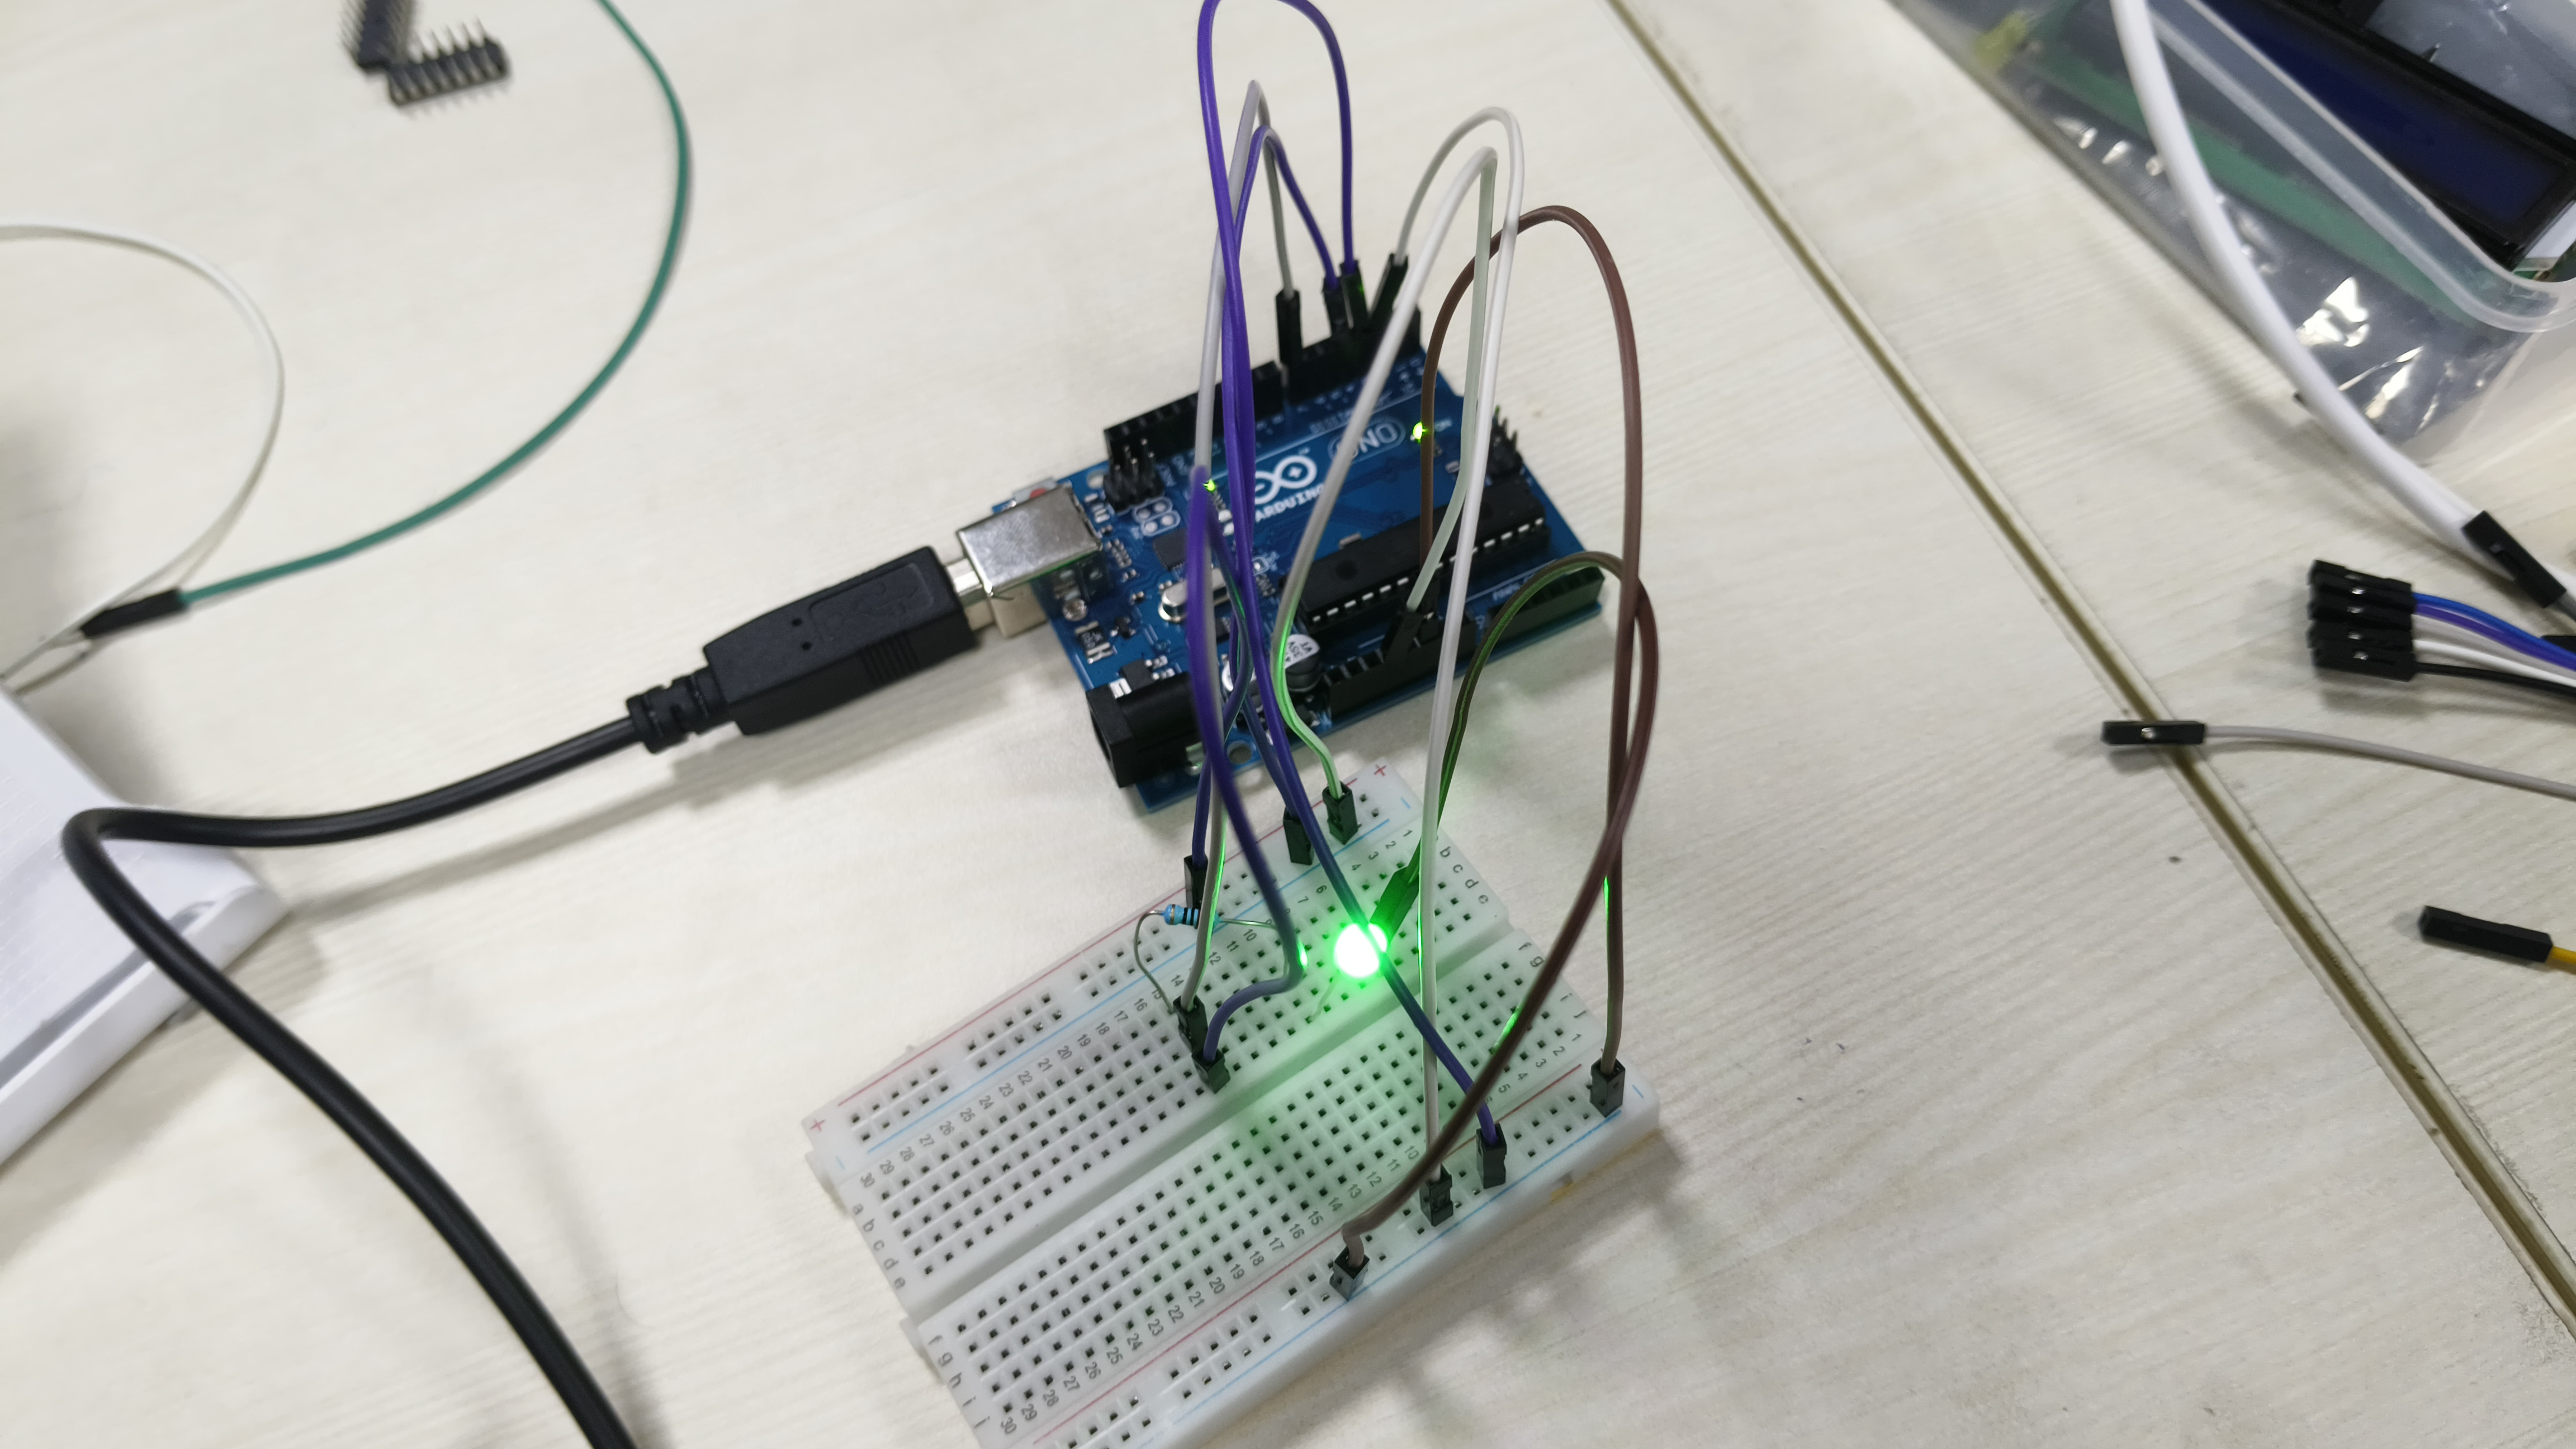
\includegraphics[width=12cm, height=12cm]{Output.jpg}
\end{center}
\section*{Conclusion}
\begin{itemize}
    	\item From Experimental Truth Table $F$ will be $1$ when $F=P.Q+Q.\overline{R}+P.\overline{R}$. 
	\item This matches option (A) from the original GATE question.
    	\item The hardware experiment confirms the circuit's theoretical logic.
\end{itemize}

\end{document}
